\section{Results}
\label{sec:results}

\subsection{National cohort derivation, data audit, and split-geometry pathology}
Across all 368,132 isolated-CABG records from 1,091 US surgical centers in STS ACSD v2.81, resolving parent--child skip logic (\cli{Complics == 1} gate) recovered \textbf{367,695 labeled procedures} (437 indeterminate records excluded) containing \textbf{89,337 treatment-requiring POAF events (24.30\%)}. Exhaustive column-by-column auditing purged seven early-position postoperative duration fields ahead of operative approach (\cli{LOS}, \cli{PLOS}, \cli{ORDuration}, \cli{SIDuration}, \cli{SurgtoMort}, \cli{SurgtoRead}, \cli{SurgtoSternInf}) together with perfusion durations, discharge therapies, STS calculators, and site/surgeon identifiers, retaining strictly 207 pre-incision predictors. Cluster-level multivariate anticlustering partitioned the 1,091 centers into 1,017 development hospitals ($N=346{,}454$; POAF 24.30\%) and 74 strictly unseen validation hospitals ($N=21{,}241$; 5,160 events; POAF 24.29\%; 0.0\% hospital overlap), achieving $|\mathrm{SMD}| < 0.10$ across every baseline clinical characteristic and matching all nine US Census divisions within 0.18 percentage points (Table~\ref{tab:cohort_baseline}).

\begin{table*}[t]
\centering
\tablefont
\caption{\ct{Baseline Patient, Clinical, Procedural, and Outcome Characteristics Across the National STS ACSD v2.81 Cohorts (1,091 US Surgical Centers, 2014--2017).}}
\label{tab:cohort_baseline}
\setlength{\tabcolsep}{5.0pt}
\renewcommand{\arraystretch}{1.04}
\begin{tabularx}{\textwidth}{@{}Yrrrr@{}}
\toprule
\thd{Characteristic} & \thd{Full Development} & \thd{Nested 50k Benchmark} & \thd{Unseen External Test} & \thd{SMD$^{\dagger}$} \\
 & \thd{($N=346{,}454$; 1,017 ctr)} & \thd{($N=50{,}000$; 1,017 ctr)} & \thd{($N=21{,}241$; 74 ctr)} & \thd{(Dev vs.\ Test)} \\
\midrule
\multicolumn{5}{@{}l}{\textit{Demographics and Anthropometry}} \\
\quad Age, mean $\pm$ SD, yr & 65.1 $\pm$ 10.1 & 66.4 $\pm$ 10.0 & 65.2 $\pm$ 10.1 & 0.009 \\
\quad Female sex & 87,423 (25.2\%) & 12,093 (24.2\%) & 5,172 (24.4\%) & 0.020 \\
\quad White race & 285,838 (82.5\%) & 41,977 (84.0\%) & 17,206 (81.0\%) & 0.039 \\
\quad Black race & 26,750 (7.7\%) & 3,413 (6.8\%) & 1,822 (8.6\%) & 0.031 \\
\quad Asian race & 11,889 (3.4\%) & 1,648 (3.3\%) & 842 (4.0\%) & 0.028 \\
\quad Hispanic or Latino ethnicity & 26,921 (7.8\%) & 3,583 (7.2\%) & 1,433 (6.8\%) & 0.039 \\
\quad Body-mass index, mean $\pm$ SD, kg/m$^2$ & 30.1 $\pm$ 6.0 & 30.1 $\pm$ 6.0 & 30.0 $\pm$ 6.0 & 0.014 \\
\quad Body surface area, mean $\pm$ SD, m$^2$ & 2.01 $\pm$ 0.24 & 2.02 $\pm$ 0.24 & 2.01 $\pm$ 0.24 & 0.008 \\
\addlinespace[3pt]
\multicolumn{5}{@{}l}{\textit{Preoperative Clinical Comorbidities and Cardiac Substrate}} \\
\quad Hypertension & 306,810 (88.6\%) & 44,569 (89.1\%) & 19,032 (89.6\%) & 0.033 \\
\quad Diabetes mellitus & 168,522 (48.6\%) & 24,025 (48.0\%) & 10,456 (49.2\%) & 0.012 \\
\quad Heart failure (current or prior) & 75,070 (21.7\%) & 11,333 (22.7\%) & 5,018 (23.6\%) & 0.047 \\
\quad NYHA class III or IV & 35,307 (10.2\%) & 5,449 (10.9\%) & 2,511 (11.8\%) & 0.052 \\
\quad Prior myocardial infarction & 180,339 (52.0\%) & 26,134 (52.3\%) & 10,960 (51.6\%) & 0.009 \\
\quad Chronic lung disease & 82,357 (23.8\%) & 12,200 (24.4\%) & 4,643 (21.9\%) & 0.045 \\
\quad Peripheral vascular disease & 46,703 (13.5\%) & 7,052 (14.1\%) & 2,688 (12.7\%) & 0.025 \\
\quad Cerebrovascular disease & 68,057 (19.6\%) & 10,323 (20.6\%) & 3,959 (18.6\%) & 0.025 \\
\quad Chronic kidney disease (eGFR $<60$) & 72,267 (20.9\%) & 11,068 (22.1\%) & 4,561 (21.5\%) & 0.015 \\
\quad Preoperative dialysis & 9,939 (2.9\%) & 1,435 (2.9\%) & 612 (2.9\%) & 0.001 \\
\quad Recorded preoperative AF history & 1,762 (0.5\%) & 282 (0.6\%) & 138 (0.7\%) & 0.018 \\
\quad Left ventricular EF, mean $\pm$ SD, \% & 52.4 $\pm$ 12.2 & 52.3 $\pm$ 12.3 & 52.4 $\pm$ 12.1 & 0.001 \\
\quad Serum creatinine, mean $\pm$ SD, mg/dL & 1.18 $\pm$ 1.06 & 1.19 $\pm$ 1.06 & 1.20 $\pm$ 1.10 & 0.018 \\
\quad CKD-EPI 2021 eGFR, mL/min/1.73\,m$^2$ & 77.7 $\pm$ 23.5 & 76.5 $\pm$ 23.4 & 77.1 $\pm$ 23.6 & 0.025 \\
\addlinespace[3pt]
\multicolumn{5}{@{}l}{\textit{Surgical Acuity, Anatomy, and Preoperative Medications}} \\
\quad Three-vessel coronary disease & 264,116 (76.2\%) & 38,363 (76.7\%) & 16,465 (77.5\%) & 0.031 \\
\quad Elective operative status & 129,234 (37.3\%) & 18,690 (37.4\%) & 7,887 (37.1\%) & 0.004 \\
\quad Urgent operative status & 202,366 (58.4\%) & 29,130 (58.3\%) & 12,439 (58.6\%) & 0.003 \\
\quad Emergent or salvage status & 14,810 (4.3\%) & 2,173 (4.3\%) & 910 (4.3\%) & 0.001 \\
\quad Preoperative $\beta$-blocker therapy & 312,486 (90.2\%) & 45,027 (90.0\%) & 18,507 (87.1\%) & 0.097 \\
\quad Preoperative amiodarone therapy & 21,722 (6.3\%) & 2,935 (5.9\%) & 1,120 (5.3\%) & 0.043 \\
\addlinespace[3pt]
\multicolumn{5}{@{}l}{\textit{Primary Outcome (Treatment-Requiring New-Onset POAF)}} \\
\quad \textbf{POAF events (STS \texttt{COtAFib})} & \textbf{84,177 (24.30\%)} & \textbf{25,000 (50.0\%)} & \textbf{5,160 (24.29\%)} & \textbf{0.0002} \\
\bottomrule
\end{tabularx}
\par\smallskip\raggedright\fontsize{7.5}{9.4}\selectfont\color{sub}
$^{\dagger}$Standardized mean difference (SMD) comparing the natural-prior full development cohort (1,017 hospitals) with the strictly hospital-disjoint unseen external validation cohort (74 hospitals; 0.0\% hospital overlap). Every clinical characteristic exhibits $|\mathrm{SMD}| < 0.10$, and all nine US Census divisions match within 0.18 percentage points. The nested 50,000-patient benchmark is class-balanced (25,000 POAF / 25,000 controls) strictly within the same 1,017 development hospitals and recalibrated back to natural clinical prevalence using the development-only Bayes offset ($-1.1365$).
\end{table*}


Center-level POAF incidence varied nearly threefold across the 928 hospitals contributing $\ge 100$ procedures, spanning 12.2\% at the 5th percentile to 34.2\% at the 95th percentile (median 24.1\%, SD~6.68~pp; Fig.~\ref{fig:study_design}b). Auditing five partition geometries showed why conventional calendar-2017 holdouts ($N=61{,}552$, 99.5\% hospital overlap) overstate external generalization: an identical 207-feature CatBoost model scored ROC-AUC 0.6778 on default calendar-2017 cases (seen centers) yet dropped $-1.99$ AUC points to \textbf{0.6579} on 2017 procedures at strictly unseen hospitals ($n=3{,}555$, 63 centers; Fig.~\ref{fig:study_design}c). Multivariate anticlustering reduced worst-case covariate imbalance 3.5-fold ($\mathrm{Max}\,|\mathrm{SMD}|$: $0.3572 \to 0.1028$) and 32-D Energy Distance 4.1-fold ($0.01732 \to 0.00427$) relative to random hospital grouping.

\subsection{Dual-paradigm modeling breaks the 50,000-patient binary ceiling across unseen hospitals}
On strictly unseen external validation ($N=21{,}241$, 74 unseen hospitals, 207 raw pre-incision predictors; Table~\ref{tab:primary_results}; Fig.~\ref{fig:primary_benchmark}), calibrated bedside risk scores showed limited discrimination: HATCH 0.5737 (95\% 74-hospital cluster CI, 0.5640--0.5839), $\mathrm{CHA_2DS_2\text{-}VASc}$ 0.5753 (0.5658--0.5845), COM-AF 0.5760 (0.5659--0.5863), Mariscalco POAF 0.6190 (0.6102--0.6281), age alone 0.6397 (0.6292--0.6503), and preoperative Mathew proxy 0.6451 (0.6344--0.6558). Six frontier 50,000-patient binary tabular model families clustered tightly between 0.6712 and 0.6746: Google TabFM v1.0.0 (0.6712), NVIDIA KumoTabular-Large v2 (0.6715), XGBoost (0.6736), LightGBM (0.6736), PriorLabs TabPFN-3.5 native 50k (0.6738), CatBoost 50k (0.6742), and Binary FT-Transformer (0.6746).

\begin{table*}[t]
\centering
\tablefont
\caption{\ct{Primary External Validation Across 74 Strictly Unseen US Surgical Centers ($N=21{,}241$; 5,160 POAF Events; 207 Raw Pre-Incision Predictors).}}
\label{tab:primary_results}
\setlength{\tabcolsep}{3.4pt}
\renewcommand{\arraystretch}{1.05}
\begin{tabularx}{\textwidth}{@{}L{1.55cm}Yrrrrrrr@{}}
\toprule
\thd{Class} & \thd{Model / Clinical Score} & \thd{ROC-AUC (95\% CI)} & \thd{AP} & \thd{ECE} & \thd{Slope} & \thd{O:E} & \thd{D10 Lift} & \thd{Fusion $\Delta$ bps (95\% CI)} \\
\midrule
\multicolumn{9}{@{}l}{\textit{Validated Bedside Clinical Risk Scores (Calibrated on 50k Development Set)}} \\
Clinical & HATCH Score & 0.5737 (0.5640--0.5839) & 0.2872 & 0.0060 & 1.006 & 0.994 & 1.45$\times$ & +1029.3 [+953.5, +1109.9]$^{\ast}$ \\
Clinical & $\mathrm{CHA_2DS_2\text{-}VASc}$ Score & 0.5753 (0.5658--0.5845) & 0.2835 & 0.0058 & 1.084 & 0.996 & 1.33$\times$ & +1013.5 [+927.2, +1105.0]$^{\ast}$ \\
Clinical & Burgos COM-AF Score & 0.5760 (0.5659--0.5863) & 0.2843 & 0.0068 & 1.067 & 0.993 & 1.38$\times$ & +1006.3 [+927.3, +1095.3]$^{\ast}$ \\
Clinical & Mariscalco POAF Score & 0.6190 (0.6102--0.6281) & 0.3097 & 0.0190 & 0.962 & 1.004 & 1.67$\times$ & +577.0 [+495.6, +656.9]$^{\ast}$ \\
Clinical & Continuous Age Alone & 0.6397 (0.6292--0.6503) & 0.3367 & 0.0127 & 0.955 & 0.996 & 1.61$\times$ & +369.6 [+290.4, +449.0]$^{\ast}$ \\
Clinical & Preoperative Mathew Proxy & 0.6451 (0.6344--0.6558) & 0.3435 & 0.0097 & 0.965 & 0.997 & 1.63$\times$ & +316.1 [+245.1, +386.1]$^{\ast}$ \\
\midrule
\multicolumn{9}{@{}l}{\textit{World-Leading Binary Tabular Foundation Models and GBDTs ($N=50{,}000$, 207 Raw Predictors)}} \\
Tabular FM & Google TabFM v1.0.0 (5$\times$10k) & 0.6712 (0.6628--0.6805) & 0.3697 & 0.0090 & 0.963 & 0.992 & 1.78$\times$ & +55.3 [+28.6, +81.5]$^{\ast}$ \\
Tabular FM & NVIDIA KumoTabular-L v2 (5$\times$10k) & 0.6715 (0.6632--0.6807) & 0.3693 & 0.0070 & 1.040 & 1.004 & 1.79$\times$ & +52.0 [+21.6, +83.3]$^{\ast}$ \\
GBDT & XGBoost (5-fold tuned) & 0.6736 & 0.3722 & 0.0069 & 0.998 & 0.992 & 1.81$\times$ & --- \\
GBDT & LightGBM (5-fold tuned) & 0.6736 & 0.3725 & 0.0060 & 1.003 & 0.993 & 1.80$\times$ & --- \\
Tabular FM & PriorLabs TabPFN-3.5 (50k native) & 0.6738 (0.6659--0.6827) & 0.3728 & 0.0068 & 1.002 & 1.002 & 1.83$\times$ & +29.2 [+8.2, +53.5]$^{\ast}$ \\
GBDT & CatBoost (5-fold binary ref) & 0.6742 (0.6659--0.6835) & 0.3744 & 0.0078 & 1.056 & 1.001 & 1.84$\times$ & +24.5 [+7.2, +42.2]$^{\ast}$ \\
Neural & Binary FT-Transformer (Gen-0) & 0.6746 (0.6664--0.6838) & 0.3756 & 0.0054 & 1.026 & 0.996 & 1.84$\times$ & +20.3 [+2.4, +38.2]$^{\ast}$ \\
\midrule
\multicolumn{9}{@{}l}{\textit{Proposed Evolutionary Target Learning, Parallel GP, and Dual-Paradigm Fusion ($N=50{,}000$, 207 Raw)}} \\
Evolved Tree & CatBoost CE (Gen-20 $z^*$) & 0.6754 & 0.3750 & 0.0084 & 0.957 & 0.995 & 1.85$\times$ & --- \\
Nested $z^*$ & EvoTarget-FT (Strictly Nested 207) & 0.6759 & 0.3764 & 0.0074 & 1.008 & 0.995 & 1.86$\times$ & --- \\
Parallel GP & JAIN Ultra GP v2 (6-family binary) & 0.6756 (0.6673--0.6850) & 0.3758 & 0.0080 & 1.002 & 0.991 & 1.85$\times$ & --- \\
Gen-0 Blend & Fair Fusion (GP v2 $+$ Binary FT) & 0.6762 & 0.3767 & 0.0046 & 1.012 & 0.993 & 1.84$\times$ & --- \\
Evolved Attn & EvoTarget-FT (Gen-20 $z^*$) & 0.6765 (0.6685--0.6856) & 0.3775 & 0.0085 & 0.976 & 0.996 & 1.85$\times$ & +1.4 [-4.0, +6.9] \\
\rowcolor{primarytint} \textbf{Champion} & \textbf{Dual-Paradigm Fusion (GP v2 $+$ FT)} & \textbf{0.6767 (0.6686--0.6858)} & \textbf{0.3777} & \textbf{0.0072} & \textbf{0.983} & \textbf{0.994} & \textbf{1.84$\times$} & \textbf{Reference} \\
\midrule
\multicolumn{9}{@{}l}{\textit{Full National Registry Data-Scale Reference ($7\times$ Larger Training Cohort, $N=346{,}454$)}} \\
7$\times$ Ref & CatBoost Full Registry (346k, 207 raw) & 0.6773 (0.6695--0.6862) & 0.3776 & 0.0076 & 1.023 & 1.000 & 1.84$\times$ & --- \\
\bottomrule
\end{tabularx}
\par\smallskip\raggedright\fontsize{7.4}{9.2}\selectfont\color{sub}
All models consume strictly the same 207 raw pre-incision predictors and are calibrated to natural clinical prevalence via uniform fold-OOF Platt scaling plus the development-only Bayes offset ($-1.1365$; zero test-label contact). Confidence intervals reflect 5,000 whole-hospital cluster bootstrap draws across all 74 unseen hospitals. $^{\ast}$95\% hospital-cluster CI strictly excludes zero. Dual-Paradigm Fusion recovers 79.2\% of the 7$\times$ 50k$\to$346k CatBoost gap while exceeding 346k CatBoost in Average Precision (0.3777 vs.\ 0.3776), 15-bin ECE (0.0072 vs.\ 0.0076), 2017 unseen-hospital AUC (0.6579 vs.\ 0.6578), and rare clinical tails (0.6935 vs.\ 0.6928), and strictly outperforming a 3-way binary neural--GBDT--TabPFN blend ($+9.9$ bps $[+0.6, +19.7]$).
\end{table*}


\begin{figure*}[t]
  \centering
  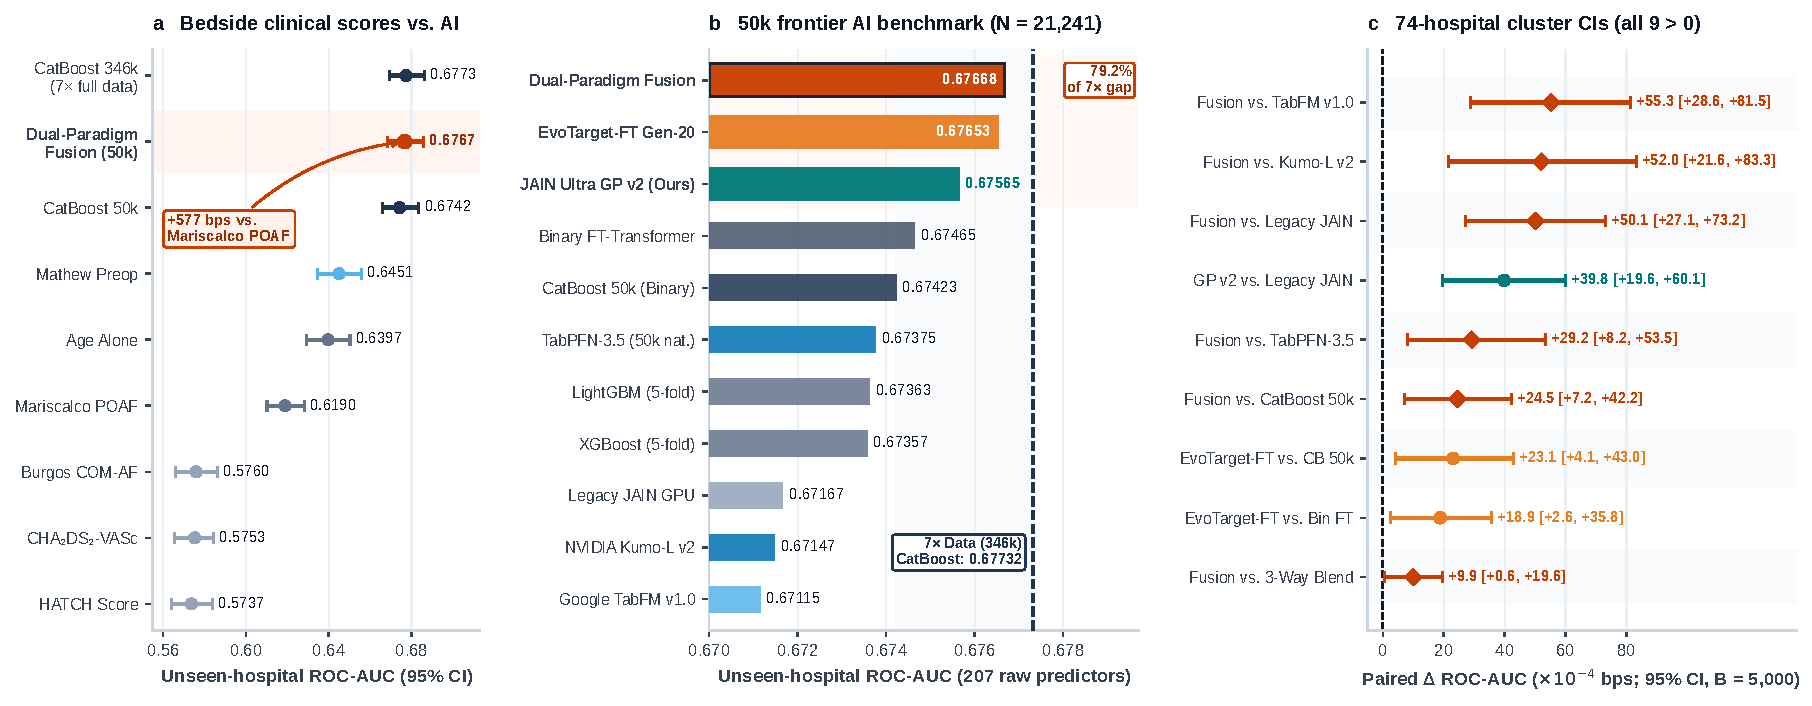
\includegraphics[width=\textwidth]{figures/fig2_primary_benchmark_and_forest.pdf}
  \caption{\ct{Unseen-hospital external validation across 74 US surgical centers ($N=21{,}241$, 207 raw predictors).} \textbf{a},~ROC-AUC comparison of six bedside clinical scores, six 50k binary tabular model families, the proposed evolutionary and parallel-GP models, and the 7$\times$-larger 346k national CatBoost reference. \textbf{b},~Paired 5,000-draw 74-hospital cluster bootstrap contrasts ($\Delta$ ROC-AUC in basis points, $\times 10^{-4}$); filled diamonds denote 95\% CIs strictly excluding zero.}
  \label{fig:primary_benchmark}
\end{figure*}

Both proposed frameworks exceeded the 50k binary band on identical 207 raw inputs: \textbf{JAIN Ultra GP v2} reached 0.6756 (0.6673--0.6850; AP~0.3758), \textbf{EvoTarget-FT} (Gen-20 $z^*$) reached 0.6765 (0.6685--0.6856; AP~0.3775), and their development-OOF \textbf{Dual-Paradigm Fusion} achieved \textbf{0.6767 (0.6686--0.6858; AP~0.3777; 15-bin ECE~0.0072; top-decile lift 1.84$\times$)}. Under 5,000-draw 74-hospital cluster bootstrapping (Fig.~\ref{fig:primary_benchmark}b), Fusion surpassed all clinical comparators---$+577.0$ bps ($[+495.6, +656.9]$) over Mariscalco POAF, $+369.6$ bps ($[+290.4, +449.0]$) over age alone, $+316.1$ bps ($[+245.1, +386.1]$) over Mathew proxy, and $>1{,}000$ bps over COM-AF, $\mathrm{CHA_2DS_2\text{-}VASc}$, and HATCH---and beat every 50k binary AI comparator with 95\% cluster CIs strictly $>0$: $+55.3$ bps ($[+28.6, +81.5]$) over TabFM, $+52.0$ bps ($[+21.6, +83.3]$) over KumoTabular-Large, $+50.1$ bps ($[+27.1, +73.2]$) over legacy JAIN GPU, $+29.2$ bps ($[+8.2, +53.5]$) over TabPFN-3.5, $+24.5$ bps ($[+7.2, +42.2]$) over CatBoost 50k, $+20.3$ bps ($[+2.4, +38.2]$) over Binary FT, and $+9.9$ bps ($[+0.6, +19.7]$, $P>0=0.982$) over a 3-way binary neural--GBDT--TabPFN blend (0.6757). Fusion recovered \textbf{79.2\%} of the 7$\times$ 50k$\to$346k CatBoost gap (0.6773) while outperforming 346k CatBoost in AP (0.3777 vs.\ 0.3776), ECE (0.0072 vs.\ 0.0076), 2017 unseen-hospital AUC (0.6579 vs.\ 0.6578), and rare clinical tails (0.6935 vs.\ 0.6928), with identical performance after excluding recorded preoperative AF ($n=21{,}103$; AUC~0.6771).

\subsection{Continuous target evolution is stable over 1,000 generations and transfers across all seven model families}
Tracking Stage-1 target evolution across 1,000 generations (256,000 teacher fits; Fig.~\ref{fig:target_evolution}a) confirmed rapid early denoising and asymptotic stability without collapse: EvoTarget-FT climbed from 0.67465 (Gen~0) to 0.67633 (Gen~10; $+16.8$ bps $[+6.2, +28.1]$) and peaked at \textbf{0.67654} at Gen~20 ($+18.9$ bps $[+2.6, +35.8]$), remaining elevated at 0.67592 through Gen~1,000 (CatBoost CE: $0.67408 \to 0.67538$ at Gen~20 $\to 0.67511$ at Gen~1,000). Replacing binary labels with Gen-20 continuous targets $z^*$ lifted unseen-hospital discrimination across \textbf{all seven independent architectures} (Fig.~\ref{fig:target_evolution}b): TabFM Reg $+97.2$ bps ($[+63.7, +132.7]$, beating binary TabFM Cls by $+26.7$ bps $[+3.7, +49.8]$), KumoTabular Reg $+27.9$ bps ($[+6.0, +51.5]$, beating binary Kumo Cls by $+35.2$ bps $[+9.0, +63.5]$), TabPFN-3.5 $5\times 10\text{k}$ Reg $+26.1$ bps ($[+6.0, +48.8]$; native 50k Reg $+13.1$ bps), EvoTarget-FT $+18.9$ bps ($[+2.6, +35.8]$), CatBoost $+12.9$ bps ($[+0.1, +26.0]$), XGBoost $+12.9$ bps, and LightGBM $+12.7$ bps.

\begin{figure*}[t]
  \centering
  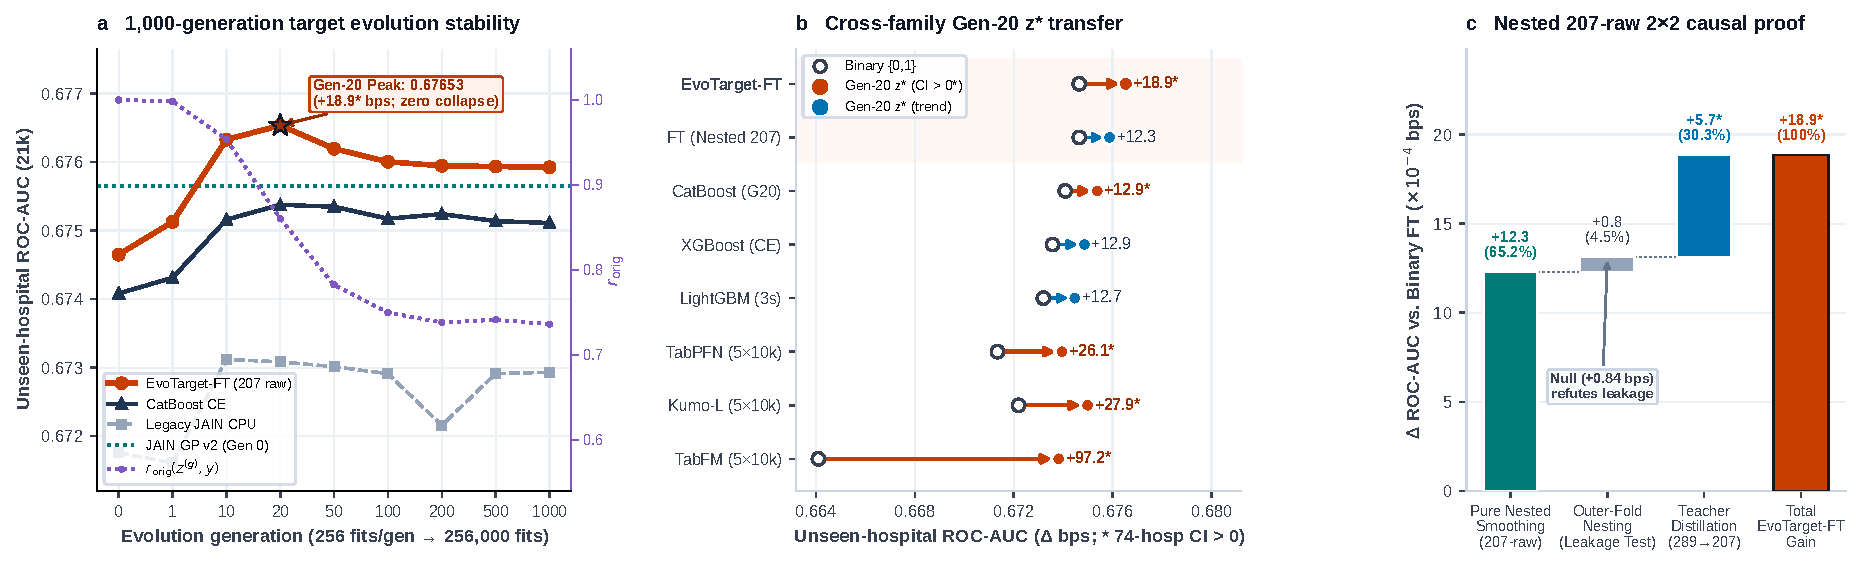
\includegraphics[width=\textwidth]{figures/fig3_target_evolution_and_causal_proof.pdf}
  \caption{\ct{1,000-generation target evolution, cross-architecture transfer, and strictly nested 2$\times$2 causal decomposition.} \textbf{a},~Unseen-hospital ROC-AUC from Gen~0 to Gen~1,000 (256,000 fits), showing a Gen-20 peak and non-collapsing plateau. \textbf{b},~Universal unseen-hospital lift when training seven distinct tabular architectures on Gen-20 continuous targets $z^*$ vs.\ binary labels (five of seven 74-hospital CIs strictly $>0$). \textbf{c},~Exact 2$\times$2 decomposition isolating strictly nested 207-raw denoising ($+12.3$ bps), null outer-fold overlap ($+0.8$ bps, $P=0.68$), and Stage-1 privileged teacher-feature distillation ($+5.7$ bps $[+0.3, +10.6]$).}
  \label{fig:target_evolution}
\end{figure*}

The strictly nested 2$\times$2 causal audit partitioned EvoTarget-FT's $+18.85$-bp lift cleanly (Fig.~\ref{fig:target_evolution}c): strictly nested 5-fold outer-loop target evolution on strictly 207 raw inputs reached \textbf{0.67588} ($+12.29$ bps $[-3.25, +28.53]$, $P>0=0.942$, 65\% of total gain); shifting from nested to global 207-raw search added a negligible $+0.84$ bps ($[-2.43, +4.40]$, $P>0=0.682$); and Stage-1 privileged distillation of 82 clinical features into $z^*$ while retaining strictly 207 raw Stage-2 inputs added a cluster-confirmed \textbf{$+5.72$ bps ($[+0.33, +10.61]$, $P>0=0.982$)}.

\subsection{Parallel genetic programming rescues symbolic modeling and preserves clinical face validity}
Resolving all six legacy JAIN bottlenecks lifted external GP discrimination by \textbf{$+39.8$ bps ($[+19.6, +60.1]$, $P>0=0.9998$)} from legacy GPU Gen-20 (0.6717) to the 6-family binary \textbf{JAIN Ultra GP v2} ensemble at \textbf{0.6756 (0.6673--0.6850)} (Fig.~\ref{fig:gp_v2_interp}a), outperforming TabFM ($+45.0$ bps $[+22.6, +69.1]$) and KumoTabular ($+41.8$ bps $[+14.0, +71.8]$) standalone. Binary-$y$ early stopping rescued soft-target GP by $+9.1$ bps ($[+0.5, +18.0]$), while fresh-seed 7-fold hospital-grouped CV ($r=0.959$ across Gen-0 pipelines) exposed $+55$-bp tree-to-tree OOF optimism on global $z^*$ that explained why binary-$y$ GP transported best (Fig.~\ref{fig:gp_v2_interp}b). Even without target evolution, combining JAIN Ultra GP v2 with Binary FT at Gen~0 achieved 0.6762 with the lowest calibration error overall (ECE~0.0046; $+15.8$ bps $[+1.0, +30.3]$ over Binary FT).

\begin{figure*}[t]
  \centering
  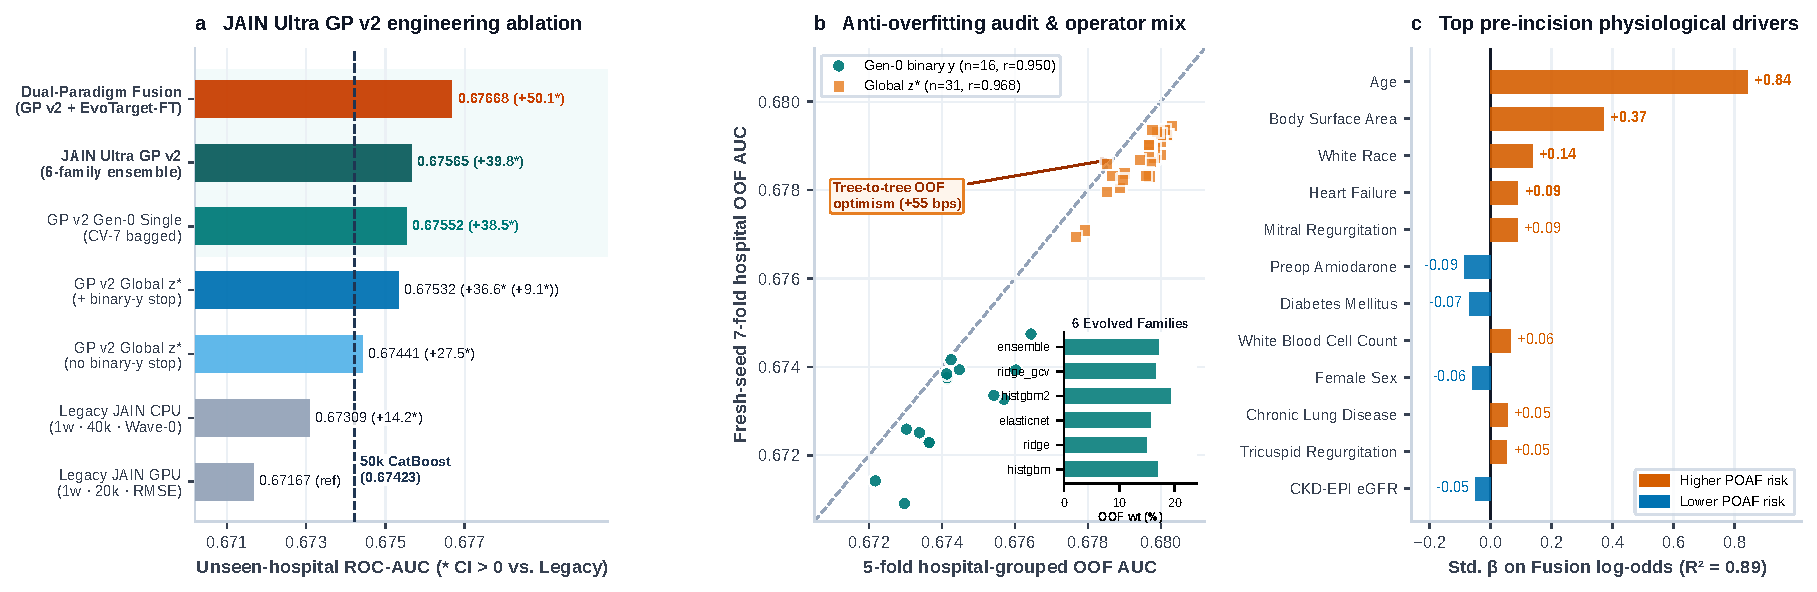
\includegraphics[width=\textwidth]{figures/fig4_jain_gp_v2_and_interpretability.pdf}
  \caption{\ct{JAIN Ultra GP v2 engineering rescue, anti-overfitting verification, and clinical drivers.} \textbf{a},~Monotonic unseen-hospital rescue from legacy JAIN GPU (0.6717) to JAIN Ultra GP v2 (0.6756, $+39.8$ bps $[+19.6, +60.1]$) and Dual-Paradigm Fusion (0.6767). \textbf{b},~Fresh-seed 7-fold vs.\ 5-fold hospital OOF audit ($r=0.959$ on binary $y$) revealing $+55$-bp tree-to-tree OOF optimism on global $z^*$, plus 6-family operator weights (inset). \textbf{c},~Top 12 standardized multivariable drivers of Fusion log-odds ($R^2 = 0.89$).}
  \label{fig:gp_v2_interp}
\end{figure*}

Log-odds from JAIN Ultra GP v2 and EvoTarget-FT exhibited high yet complementary concordance ($r=0.9591$). Multivariable standardized surrogate regression explained \textbf{89.0\%} ($R^2 = 0.8896$) of Dual-Paradigm Fusion log-odds variance with physiologically coherent pre-incision drivers (Fig.~\ref{fig:gp_v2_interp}c): age ($\beta = +0.84$), body surface area ($+0.37$), White race ($+0.14$), heart failure ($+0.09$), mitral regurgitation ($+0.09$), white blood cell count ($+0.06$), chronic lung disease ($+0.05$), and tricuspid regurgitation ($+0.05$) increased predicted risk, while preoperative amiodarone ($\beta = -0.09$), diabetes ($-0.07$), female sex ($-0.06$), and higher CKD-EPI eGFR ($-0.05$) reduced risk.

\subsection{Calibration, decile risk stratification, and Decision Curve net clinical benefit}
Recalibrated strictly via development-only fold-OOF Platt scaling and Bayes prior shift ($-1.1365$), Dual-Paradigm Fusion achieved slope \textbf{0.983}, O:E \textbf{0.994}, 15-bin ECE \textbf{0.0072}, and ICI \textbf{0.0114} across 21,241 unseen-hospital patients (Fig.~\ref{fig:calibration_dca}a). Observed POAF risk climbed monotonically across predicted deciles from \textbf{6.07\%} (5.13\%--7.17\%; 129/2,125) in D1 to \textbf{44.82\%} (42.72\%--46.94\%; 952/2,124; 1.84$\times$ enrichment) in D10, yielding a \textbf{7.4-fold} risk separation (Fig.~\ref{fig:calibration_dca}b).

\begin{figure*}[t]
  \centering
  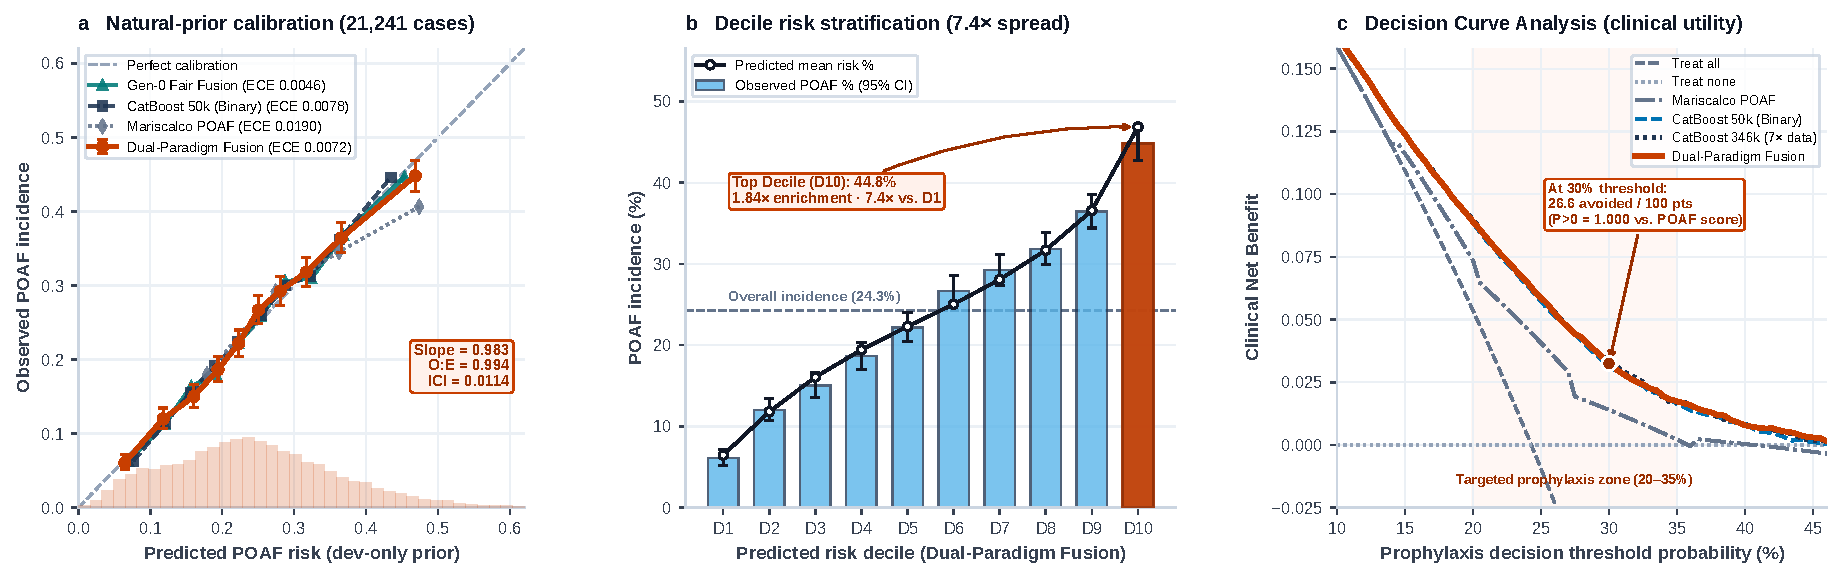
\includegraphics[width=\textwidth]{figures/fig5_calibration_stratification_dca.pdf}
  \caption{\ct{External calibration, decile risk stratification, and Decision Curve Analysis ($N=21{,}241$, 74 unseen hospitals).} \textbf{a},~Natural-prior calibration across risk deciles using strictly development-only recalibration (slope~0.983, O:E~0.994, ECE~0.0072, ICI~0.0114). \textbf{b},~Monotonic POAF incidence across Fusion deciles from 6.07\% (D1) to 44.82\% (D10; 7.4$\times$ spread). \textbf{c},~Decision Curve Net Benefit across 10\%--45\% thresholds, avoiding 20.4--33.8 unnecessary interventions per 100 patients across 25\%--35\% thresholds ($P>0=1.000$ vs.\ Mariscalco POAF).}
  \label{fig:calibration_dca}
\end{figure*}

In Decision Curve Analysis (Fig.~\ref{fig:calibration_dca}c; Supplementary Table~\ref{tab:supp_dca}), Dual-Paradigm Fusion delivered superior Net Benefit across the 15\%--40\% prophylaxis decision window. At 25\%, 30\%, and 35\% decision thresholds, Fusion flagged 45.1\%, 29.3\%, and 17.5\% of patients, achieving positive Net Benefits of \textbf{0.0587}, \textbf{0.0325}, and \textbf{0.0174} (versus $-0.0094$, $-0.0815$, and $-0.1647$ for universal prophylaxis) and avoiding \textbf{20.4}, \textbf{26.6}, and \textbf{33.8 unnecessary prophylactic interventions per 100 patients}, outperforming Mariscalco POAF with cluster bootstrap $P>0 = 1.000$ at every threshold from 15\% to 35\%.

\subsection{Subgroup equity and center-level transport across 74 unseen hospitals}
Dual-Paradigm Fusion outperformed Mariscalco POAF across all 25 prespecified demographic, clinical, acuity, stress-slice, and hospital-volume subgroups ($+374.0$ to $+1{,}332.5$ bps) and beat CatBoost 50k in \textbf{24 of 25 subgroups} (Fig.~\ref{fig:equity_transport}a; Supplementary Table~\ref{tab:supp_subgroups}), maintaining strong discrimination and calibration in female (0.6891, $+37.2$ bps), male (0.6719), Black (0.6849, O:E~1.034), Hispanic/Latino (0.7146), diabetic (0.6812), low-LVEF (0.6787), urgent/emergent (0.6830, $+35.8$ bps), rare-tail (0.6935, $+44.7$ bps), and low-, mid-, and high-volume center strata (0.6818, 0.6851, and 0.6727).

\begin{figure*}[t]
  \centering
  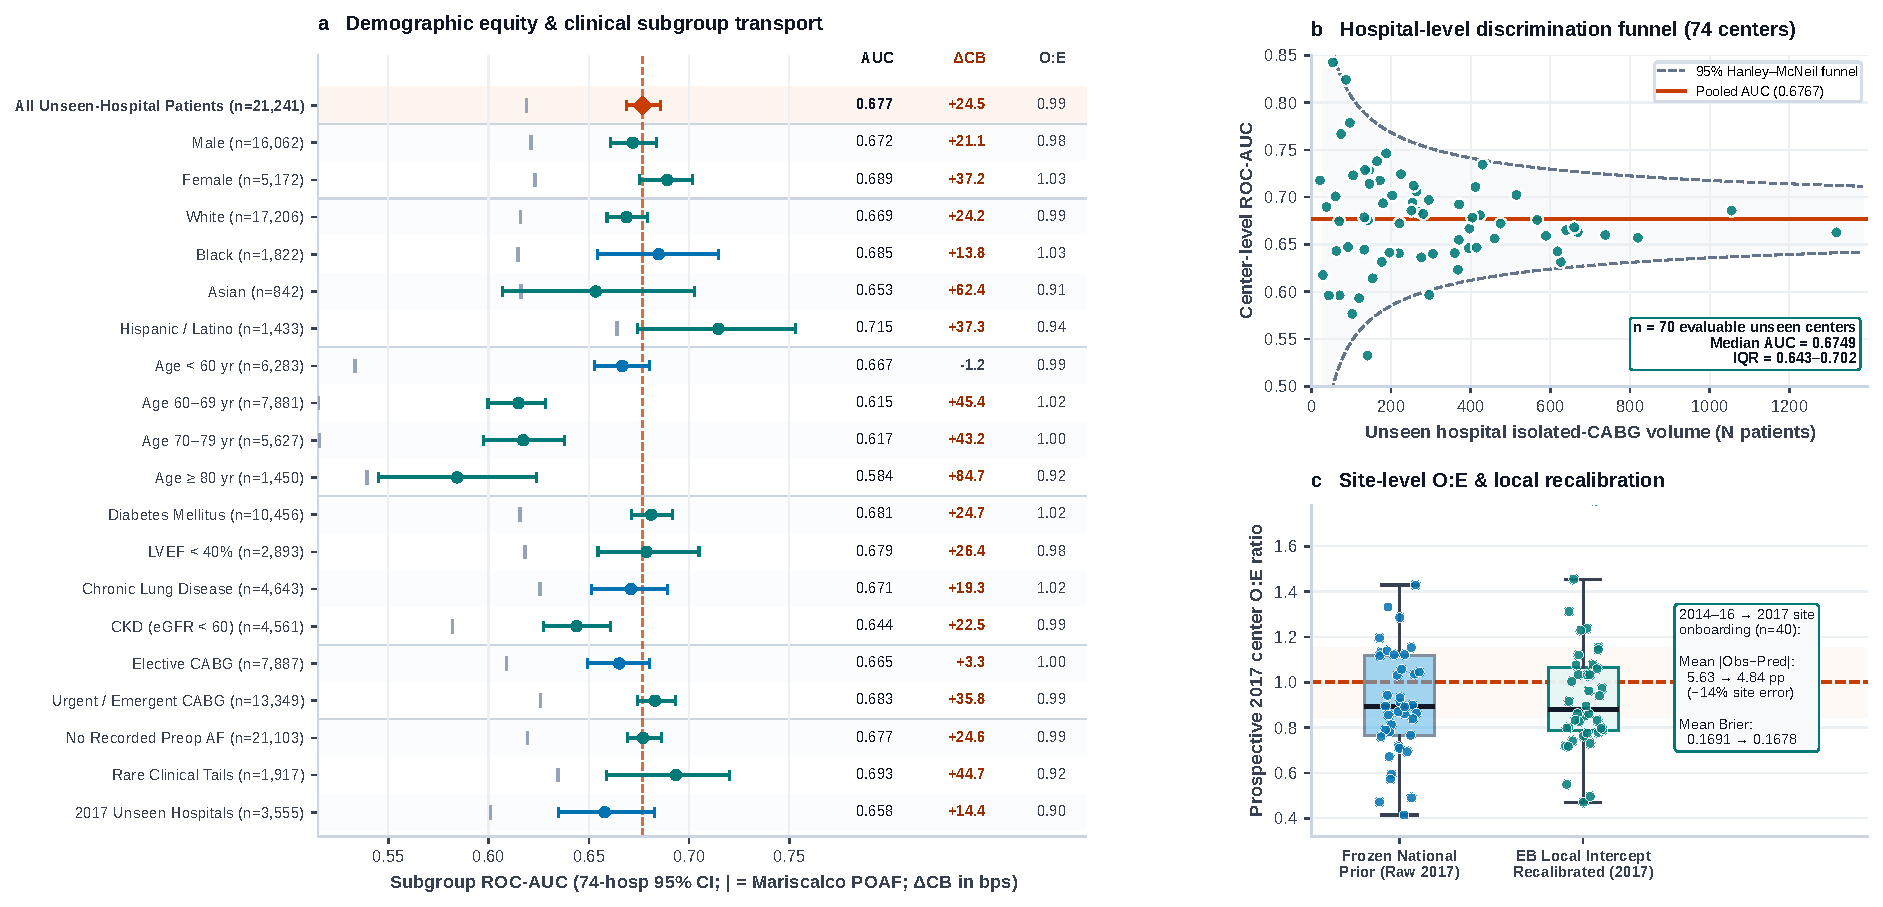
\includegraphics[width=\textwidth]{figures/fig6_equity_subgroups_and_hospital_transport.pdf}
  \caption{\ct{Subgroup equity audit, 74-hospital discrimination funnel, and chronological local intercept recalibration.} \textbf{a},~Subgroup ROC-AUC (74-hospital 95\% CIs), $\Delta$ vs.\ CatBoost 50k (bps), and O:E across prespecified strata (ticks mark Mariscalco POAF). \textbf{b},~Center-level ROC-AUC across 70 evaluable unseen hospitals inside the 95\% Hanley--McNeil funnel (median AUC~0.6749, IQR~0.6434--0.7021). \textbf{c},~Chronological 2014--2016$\to$2017 empirical-Bayes site intercept updating ($m_0=100$, $n=40$ centers), cutting center-level mean absolute rate error by 14\% (5.63 $\to$ 4.84~pp) and improving Brier score (0.1691 $\to$ 0.1678).}
  \label{fig:equity_transport}
\end{figure*}

Across the 70 evaluable unseen centers, hospital-level AUC conformed tightly to the 95\% Hanley--McNeil funnel (median \textbf{0.6749}, IQR 0.6434--0.7021; Fig.~\ref{fig:equity_transport}b), whereas raw center-level O:E ratios reflected institutional incidence dispersion (median 0.958, IQR 0.856--1.135 for $n \ge 50$). Updating a single empirical-Bayes local intercept ($m_0=100$) from each center's 2014--2016 procedures prior to 2017 deployment ($n=40$ centers; Fig.~\ref{fig:equity_transport}c) reduced center-level mean absolute POAF rate error by \textbf{14\%} (5.63 $\to$ 4.84~pp) and improved Brier score from 0.16914 to 0.16777.

\subsection{Seen-hospital deployment reveals implicit site familiarity and a 180-bp empirical-Bayes calibration gain}
To separate institutional familiarity from temporal drift and quantify in-network health-system deployment, we trained and evaluated every algorithm on the matched \textbf{100.0\% Seen-Hospital} partition guaranteeing all 1,091 US surgical centers appear in both the 346,454-case development cohort and the nested 50,000-case balanced training benchmark (zero patient overlap; matched natural-prior holdout $N=21{,}241$ across 1,086 seen centers, 0 unseen centers; Table~\ref{tab:seen_vs_unseen}; Fig.~\ref{fig:seen_vs_unseen}).

\begin{table*}[t]
\centering\tablefont
\caption{\ct{Head-to-Head Transport Audit: Unseen-Hospital Cold Start (0\% Overlap, 74 Centers) vs.\ Seen-Hospital In-Network Deployment (100\% Overlap, All 1,091 Centers in Training; $N=21{,}241$ Natural-Prior Holdout).}}
\label{tab:seen_vs_unseen}
\setlength{\tabcolsep}{4.0pt}
\renewcommand{\arraystretch}{1.05}
\begin{tabularx}{\textwidth}{@{}Yrrrrrr@{}}
\toprule
\thd{Model Family} & \thd{Unseen Hosp.} & \thd{Seen Hosp.} & \thd{Seen + 50k} & \thd{Seen + 346k} & \thd{Site-Prior} & \thd{In-Net} \\
 & \thd{(0\% ovlp, 207)} & \thd{(100\%, 207 raw)} & \thd{EB Site Prior} & \thd{EB Site Prior} & \thd{Gain (bps)} & \thd{ECE} \\
\midrule
Mariscalco POAF Score & 0.6190 & 0.6276 & --- & --- & --- & 0.0166 \\
Google TabFM v1.0.0 (5$\times$10k) & 0.6712 & 0.6775 & 0.6918 & 0.6986 & +210 & 0.0093 \\
NVIDIA KumoTabular-L v2 (5$\times$10k) & 0.6715 & 0.6764 & 0.6911 & 0.6977 & +213 & 0.0080 \\
XGBoost (5-fold binary) & 0.6736 & 0.6774 & 0.6895 & 0.6958 & +184 & 0.0100 \\
LightGBM (5-fold binary) & 0.6736 & 0.6780 & 0.6897 & 0.6960 & +180 & 0.0084 \\
PriorLabs TabPFN-3.5 (50k native) & 0.6738 & 0.6795 & 0.6919 & 0.6982 & +187 & 0.0086 \\
CatBoost 50k (5-fold binary) & 0.6742 & 0.6777 & 0.6902 & 0.6966 & +188 & 0.0089 \\
Binary FT-Transformer (Gen-0) & 0.6746 & 0.6784 & 0.6890 & 0.6958 & +174 & 0.0067 \\
JAIN Ultra GP v2 (6-family) & 0.6756 & 0.6788 & 0.6904 & 0.6969 & +181 & 0.0098 \\
EvoTarget-FT (Gen-20 $z^*$) & 0.6765 & 0.6793 & 0.6906 & 0.6972 & +179 & 0.0117 \\
\rowcolor{primarytint} \textbf{Dual-Paradigm Fusion (GP v2 $+$ FT)} & \textbf{0.6767} & \textbf{0.6794} & \textbf{0.6909} & \textbf{0.6974} & \textbf{+180} & \textbf{0.0110} \\
CatBoost Full Registry (346k, 7$\times$) & 0.6773 & 0.6831 & --- & 0.7014 & +183 & 0.0083 \\
\bottomrule
\end{tabularx}
\par\smallskip\raggedright\fontsize{7.4}{9.2}\selectfont\color{sub}
In the Seen-Hospital benchmark, every one of the 1,091 US surgical centers appears in both the 346,454-case full development set and the nested 50,000-case balanced benchmark (100.0\% hospital overlap; zero unseen test centers; exact matched $N=21{,}241$ holdout with 24.30\% POAF prevalence). Empirical-Bayes (EB) hospital incidence priors are computed strictly from training rows with zero test-label exposure.
\end{table*}


\begin{figure*}[t]
  \centering
  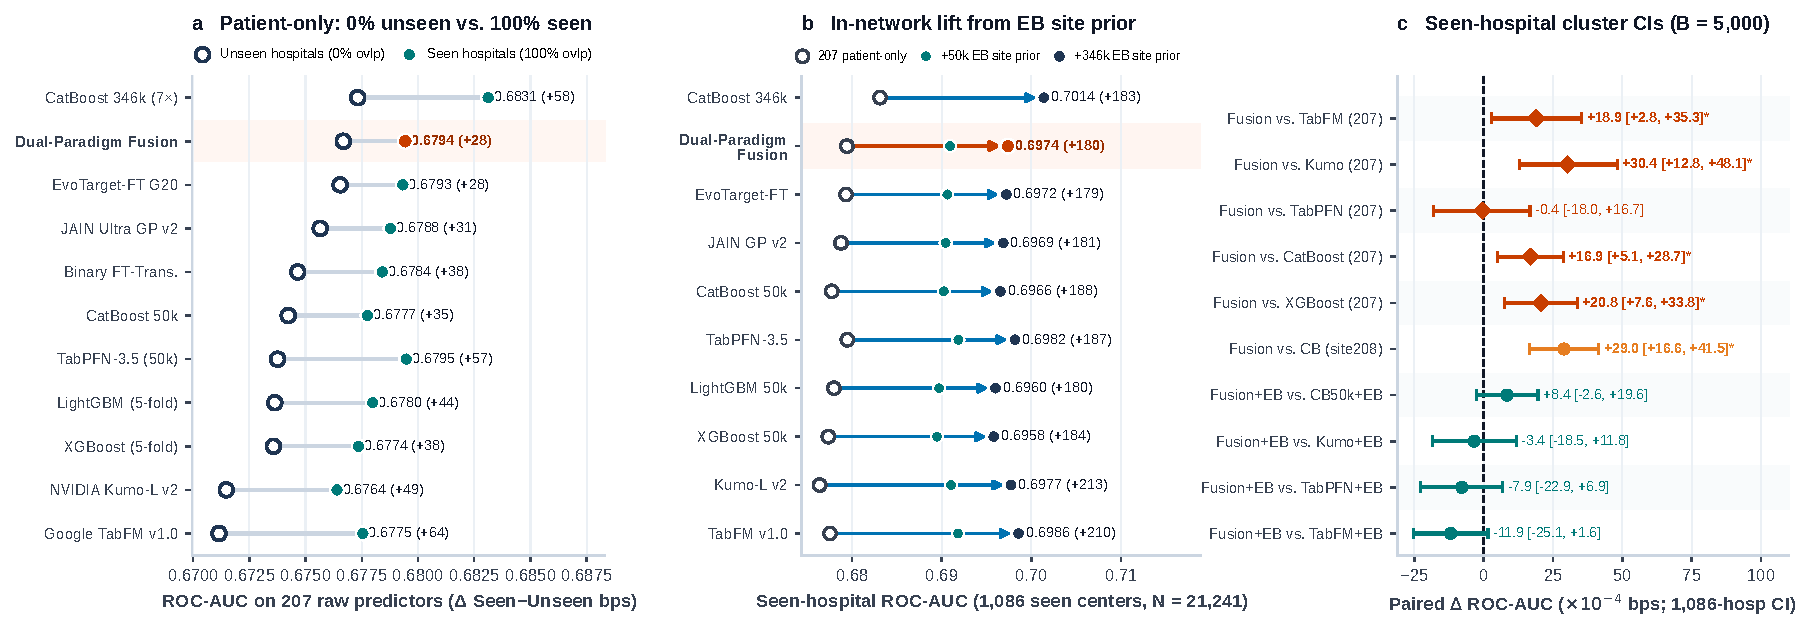
\includegraphics[width=\textwidth]{figures/fig7_seen_vs_unseen_hospitals.pdf}
  \caption{\ct{Unseen-hospital cold start (0\% overlap) versus seen-hospital in-network deployment (100\% all-1,091-hospitals-in-train; $N=21{,}241$).} \textbf{a},~Patient-only ROC-AUC on strictly 207 raw predictors (zero hospital identifiers), showing a universal $+28$--$64$-bp familiarity inflation with larger shifts for tabular foundation models ($+49$--$64$ bps) than Dual-Paradigm Fusion ($+28$ bps). \textbf{b},~Closed-form train-only empirical-Bayes hospital priors lift every 50k model by $+174$--$213$ bps (to 0.696--0.699) and push 346k CatBoost to 0.7014. \textbf{c},~Paired 5,000-draw 1,086-hospital cluster bootstrap contrasts ($\Delta$ ROC-AUC in bps; asterisks indicate 95\% CIs strictly $>0$).}
  \label{fig:seen_vs_unseen}
\end{figure*}

Three major findings emerged across the 1,086 seen hospitals. First, on strictly \textbf{207 raw patient-only predictors without hospital identifiers} (Fig.~\ref{fig:seen_vs_unseen}a), seeing all 1,091 hospitals in training lifted every model by \textbf{$+28$ to $+64$ bps} relative to unseen hospitals, confirming that hospital overlap alone inflates apparent external validation by 0.3--0.6 AUC points. Tabular foundation models exhibited the largest seen-hospital jumps---Google TabFM ($5\times 10\text{k}$, 40 NNLS estimators) $+64$ bps ($0.6712 \to 0.6775$), TabPFN-3.5 native 50k $+57$ bps ($0.6738 \to 0.6795$), and KumoTabular-Large $+49$ bps ($0.6715 \to 0.6764$), alongside CatBoost 346k ($+58$ bps, $0.6773 \to 0.6831$). Dual-Paradigm Fusion (Regime-1 locked weights, zero test peeking) rose only $+28$ bps ($0.6767 \to \mathbf{0.6794}$, 95\% 1,086-hospital CI 0.6716--0.6874) and JAIN Ultra GP v2 rose $+31$ bps ($0.6756 \to 0.6788$), indicating roughly half the unseen-hospital shrinkage of tabular foundation models while strictly outperforming KumoTabular ($+30.4$ bps $[+12.8, +48.1]$), XGBoost ($+20.8$ bps $[+7.6, +33.8]$), TabFM ($+18.9$ bps $[+2.8, +35.3]$), CatBoost 50k ($+16.9$ bps $[+5.1, +28.7]$), LightGBM ($+14.5$ bps $[+1.9, +27.5]$), and Mariscalco POAF ($+517.9$ bps $[+449.3, +586.8]$; Fig.~\ref{fig:seen_vs_unseen}c), and matching TabPFN-3.5 native 50k ($-0.4$ bps $[-18.0, +16.7]$).

Second, incorporating each center's strictly train-only Empirical-Bayes (EB) historical POAF incidence prior vaulted every architecture by \textbf{$+174$ to $+213$ bps} (nearly $+2.0$ AUC points; Fig.~\ref{fig:seen_vs_unseen}b), lifting AP from 0.386 to 0.407--0.411, top-decile enrichment to 1.94--1.96$\times$, and 30\%-threshold Net Benefit from 0.035 to 0.042--0.044. Under native end-to-end 208-feature 50k training (\cli{site208}), \textbf{Dual-Paradigm Fusion (\cli{site208})} ranked first among all native 50k models at \textbf{0.6916 (0.6844--0.6987)}, decisively beating CatBoost \cli{site208} (0.6887; \textbf{$+29.0$ bps $[+16.6, +41.5]$, $P>0=1.000$}), XGBoost \cli{site208} (0.6883), and LightGBM \cli{site208} (0.6883). Under parameter-free closed-form Bayesian hospital-intercept updating with the 346k historical hospital prior ($\operatorname{Platt}_{\mathrm{OOF}} + \text{dev offset} + \hat{\delta}_h^{\mathrm{EB}_{346\mathrm{k}}}$), every 50k model rose to \textbf{0.6958--0.6986} (Dual-Paradigm Fusion \textbf{0.6974}, $+179.6$ bps $[+149.6, +209.9]$, AP~0.4069), and full-registry 346k CatBoost (\cli{site208}) crossed 0.70 at \textbf{0.7014 (0.6942--0.7087; $+182.7$ bps $[+152.4, +212.8]$, AP~0.4109, ECE~0.0083, slope~1.014, O:E~0.999, lift 1.96$\times$)}.

Third, auditing correlations between patient-only logits and true hospital incidence deviations ($\hat{\delta}_h^{\mathrm{EB}_{346\mathrm{k}}}$) revealed \emph{implicit hospital fingerprinting}: models fit on 40,000--346,000 cases across all 1,091 hospitals absorbed moderate site-coding signatures even without \cli{HospID} (CatBoost 346k $r=+0.1431$; Dual-Paradigm Fusion $r=+0.1298$; JAIN GP v2 $r=+0.1284$; CatBoost 50k $r=+0.1216$; TabPFN-3.5 native 50k $r=+0.1184$), whereas 10,000-row bagged tabular foundation models (seeing $\sim$9 patients/hospital per shard) showed $\sim$30\% lower institutional entanglement ($r=+0.0878$--$0.0919$). When added to the explicit 346k EB hospital intercept, lower-entanglement 10k-shard TabPFN-3.5 and TabFM avoided double-counting the site effect and achieved 0.6986 versus 0.6974 for Dual-Paradigm Fusion (cluster CIs spanning zero: $-7.9$ to $-11.9$ bps).
